\ifdefined\CUMULATIVEPRACTICE
\else
\documentclass[11pt]{article}
\newcommand{\coursedocname}{Midterm Practice Problems}

\usepackage[utf8]{inputenc}
\usepackage[T1]{fontenc}
\usepackage{lmodern}
\usepackage[margin=1in]{geometry}
\usepackage[dvipsnames]{xcolor}
\usepackage{graphicx, booktabs, enumitem, float, framed, caption, multirow}
\usepackage{fancyhdr}
\usepackage{tcolorbox}
\usepackage{listings}
\usepackage{tikz}
\usepackage{setspace}
\usepackage{needspace}
\IfFileExists{algorithm.sty}{%
  \usepackage{algorithm}
  \usepackage[noend]{algpseudocode}
  \newcommand{\hasalgorithms}{}%
}{}
\usepackage{amsmath,amssymb,bm,xcolor}


\newcommand{\st}{\mathbf{x}}            %

\newcommand{\act}{a}                    %
\newcommand{\actspace}{\mathcal{A}}     %
\newcommand{\Sset}{\mathcal{S}}         %
\newcommand{\disc}{\gamma}              %
\newcommand{\Vfun}{V}                   %
\newcommand{\heur}{h}                   %

\newcommand{\Rc}{\mathbf{R}}            %

\newcommand{\bel}{\mathrm{bel}}         %

\newcommand{\rot}{\mathbf{R}}           %
\newcommand{\tra}{\mathbf{t}}           %
\newcommand{\Tf}[2]{{}^{#1}\mathbf{T}_{#2}}  %
\usepackage{hyperref}

\definecolor{DartmouthGreen}{HTML}{00693E}
\newcommand{\dgreen}[1]{\textcolor{DartmouthGreen}{#1}}
\newcommand{\dgbf}[1]{\textbf{\dgreen{#1}}}      %
\urlstyle{same}
\hypersetup{
    colorlinks=true,
    linkcolor=DartmouthGreen,
    filecolor=DartmouthGreen,
    citecolor=DartmouthGreen,
    urlcolor=DartmouthGreen,
    breaklinks=true
}

\newcommand{\coursenumber}{COSC 81/281}
\newcommand{\gradescopelink}{\textbf{Gradescope} (\url{https://www.gradescope.com/courses/1372528})}


\setlength{\parindent}{0pt}
\setlength{\parskip}{6pt plus 2pt minus 1pt}
\setlength{\headheight}{13.6pt}
\setlength{\emergencystretch}{3em}
\providecommand{\tightlist}{\setlength{\itemsep}{0pt}\setlength{\parskip}{0pt}}
\setcounter{secnumdepth}{0}

\DeclareRobustCommand{\callout}[2][gray!10]{%
  \begin{tcolorbox}[left=8pt, arc=0pt, outer arc=0pt,
                    colframe=#1, colback=#1, coltext=black]#2\end{tcolorbox}}




\newcommand{\bonusq}{\textsf{\small\textbf{[Bonus]}}~}
\newcommand{\bonus}{\bonusq}

\newcommand{\setupheader}[1]{%
  \fancypagestyle{default}{%
      \lhead{#1}
      \chead{}
      \rhead{\textbf{\coursenumber}}
      \lfoot{}
      \cfoot{}
      \rfoot{\thepage}
      \renewcommand{\headrulewidth}{0.4pt}
      \renewcommand{\footrulewidth}{0.4pt}
  }
  \pagestyle{default}
  \fancypagestyle{plain}{\pagestyle{default}}
}
\newcommand{\setupexamheader}[1]{%
  \fancypagestyle{default}{%
      \lhead{#1}
      \chead{Name:}
      \rhead{}
      \lfoot{}
      \cfoot{}
      \rfoot{\thepage}
      \renewcommand{\headrulewidth}{0.4pt}
      \renewcommand{\footrulewidth}{0.4pt}
  }
  \pagestyle{default}
  \fancypagestyle{plain}{\pagestyle{default}}
}
\newcommand{\pstitle}[2]{%
  \title{\textbf{\coursenumber:} #1}
  \author{\textbf{Due} #2\\
  }
  \date{}
}

\newcommand{\coursenotice}{%
  \callout{Problem sets are graded \textbf{pass/fail on completion}, and
  there are no late days. The problem sets are where the learning happens,
  and they are the best available practice for the midterm and final exam.
  Submit to \gradescopelink\ and assign each question to a page in your
  submission. Questions are welcome on \dgbf{Slack}. Starred ($\bigstar$)
  questions are required for COSC 281 students and optional (ungraded) for
  COSC 81 students.}}

\lstset{
  language=python,
  basicstyle=\ttfamily,
  commentstyle=\color{BrickRed},
  stringstyle=\color{ForestGreen},
  showstringspaces=false,
  breaklines=true,
  breakatwhitespace=true,
  keywordstyle=\color{Purple},
  emph={def},
  emphstyle=\color{RoyalBlue}
}
\lstnewenvironment{itemlisting}[1][]
 {\mbox{}\vspace*{-\baselineskip}%
  \lstset{xleftmargin=\leftmargin, linewidth=\linewidth, #1}}
 {}

\makeatletter
\def\fps@figure{htbp}
\makeatother
\ifdefined\hasalgorithms
\fi


\newenvironment{studentanswer}[1]
  {\par\medskip\noindent
   \begin{tcolorbox}[height from=#1 to 100cm, colback=white, colframe=gray!60,
     boxrule=0.6pt, arc=0pt, outer arc=0pt, left=7pt, right=7pt,
     top=7pt, bottom=7pt, title={Answer / work}, fonttitle=\small,
     coltitle=black, colbacktitle=gray!8, titlerule=0pt]
   \ignorespaces}
  {\end{tcolorbox}\par}

\setupheader{\coursedocname}
\begin{document}
\section*{Midterm practice problems}
This collection provides additional practice with the topics in PS1 and
PS2. It is not intended to match the length or structure of the midterm,
and it is not a timed practice exam. Work through the problems at your
own pace, using the worked solutions to examine the reasoning behind
each step after you have attempted a solution.

For some questions, several approaches may be appropriate.
Explain how the objective, available information, and constraints support
your choice.

The written problems are followed by an optional programming exercise.
This collection is for preparation, not an additional graded submission.
You may enter answers and plots in the \texttt{studentanswer} environments
of \texttt{midterm-practice/handout.tex}, or write on the PDF.
Solutions are distributed separately.

\begin{quote}\small\textbf{AI Policy.} You may use any AI tools you like to assist you with your assignments, and you should, as that is likely how you will work for the rest of your career.
That being said, the written portions are practice for the in-class midterm and exam, which are closed book and on paper. You should strive to answer these yourself and use AI as a tutor and not an oracle.
\end{quote}

\callout{Please include an AI Tool Disclosure Below \vspace{50pt}}

The formula sheet is included for reference and will be included in the exam.
\clearpage
\section*{Formula sheet}
\begingroup
\small
\setlength{\abovedisplayskip}{7pt}
\setlength{\belowdisplayskip}{7pt}
\textbf{Search and planning}
\[
 f(n)=g(n)+h(n),\quad h(n)\le h^*(n),\quad
 h(n)\le c(n,n')+h(n'),\quad h(G)=0
\]
\[
\text{Break A* ties by lower }h\text{, then row-major order.}
\]

\textbf{MDPs and RL}
\[
 (\Sset,\actspace,T,R,\gamma),\quad T(s'\mid s,a)=P(s'\mid s,a),\quad
 \sum_{s'}T(s'\mid s,a)=1,\quad 0\le\gamma<1
\]
\[
 \begin{gathered}
 Q^*(s,a)=\sum_{s'}T(s'\mid s,a)
 [R(s,a,s')+\gamma\max_{a'}Q^*(s',a')]\\[4pt]
 V^*(s)=\max_a Q^*(s,a),\qquad
 \pi^*(s)\in\arg\max_a Q^*(s,a)
 \end{gathered}
\]
\[
 V_{k+1}(s)=\max_a\sum_{s'}T(s'\mid s,a)[R(s,a,s')+\gamma V_k(s')]
\]
\[
 V^{\pi_k}(s)=\sum_{s'}T(s'\mid s,\pi_k(s))
 [R(s,\pi_k(s),s')+\gamma V^{\pi_k}(s')]
\]
\[
 \pi_{k+1}(s)\in\arg\max_a\sum_{s'}T(s'\mid s,a)[R(s,a,s')+\gamma V^{\pi_k}(s')]
\]
\[
 V(s)\leftarrow V(s)+\alpha[r+\gamma V(s')-V(s)]
\]
\[
 Q(s,a)\leftarrow Q(s,a)+\alpha[r+\gamma\max_{a'}Q(s',a')-Q(s,a)]
\]
\textbf{Optimization}
\[
 \st_{k+1}=\st_k-\alpha\nabla f(\st_k),\qquad
 f(x)\approx f(x_0)+f'(x_0)(x-x_0)+\tfrac12 f''(x_0)(x-x_0)^2
\]
\textbf{Transforms}
\[
 \Tf{a}{b}=\begin{bmatrix}\rot&\tra\\0&1\end{bmatrix},\quad
 \begin{bmatrix}p_a\\1\end{bmatrix}=\Tf{a}{b}\begin{bmatrix}p_b\\1\end{bmatrix},\quad
 \Tf{a}{c}=\Tf{a}{b}\Tf{b}{c},\quad
 R_z(\theta)=\begin{bmatrix}\cos\theta&-\sin\theta&0\\\sin\theta&\cos\theta&0\\0&0&1\end{bmatrix}
\]
\textbf{Calculus}
\[
 (x^n)'=nx^{n-1},\quad(\sin x)'=\cos x,\quad(\cos x)'=-\sin x
\]
\[
 \sin0=0,\quad\cos0=1,\quad\sin(\pi/2)=1,\quad\cos(\pi/2)=0
\]
\endgroup

\clearpage
\fi
\section*{Part 1: Written practice}
\section*{Question 1: Changing a heuristic}
The directed graph has edges $S\to A$ of cost 2, $S\to B$ of cost 1,
$B\to A$ of cost $\tfrac12$, $A\to G$ of cost 2, and $B\to G$ of cost 5.
There are no other edges. The heuristic is
$h(S)=3$, $h(A)=2$, $h(B)=1$, $h(G)=0$.
\begin{center}
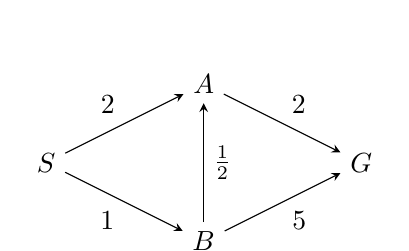
\begin{tikzpicture}[>=stealth,scale=1.0]
\node (S) at (0,0) {$S$};\node (A) at (2,1) {$A$};
\node (B) at (2,-1) {$B$};\node (G) at (4,0) {$G$};
\draw[->] (S)--node[above left]{2}(A);
\draw[->] (S)--node[below left]{1}(B);
\draw[->] (B)--node[right]{$\tfrac12$}(A);
\draw[->] (A)--node[above right]{2}(G);
\draw[->] (B)--node[below right]{5}(G);
\end{tikzpicture}
\end{center}
\begin{enumerate}[label=(\alph*)]
\item Find the optimal cost from each node to $G$. Is the
heuristic admissible? Justify by comparing the values.

\begin{studentanswer}{0.8in}
%%%%% SOLUTION HERE %%%%%
\end{studentanswer}

\item Is it consistent? Identify a specific edge inequality
that establishes your answer.

\begin{studentanswer}{0.65in}
%%%%% SOLUTION HERE %%%%%
\end{studentanswer}

\item Change only $h(B)$ to $\tfrac52$. Is the resulting
heuristic both admissible and consistent? Check all edges incident to $B$
and explain why the remaining edges do not create a new violation.

\begin{studentanswer}{0.85in}
%%%%% SOLUTION HERE %%%%%
\end{studentanswer}

\end{enumerate}

\clearpage
\section*{Question 2: Validating an RRT extension}
A two-dimensional configuration-space RRT currently contains nodes
$q_0=(0,0)$ and $q_1=(0,2)$. The next sample is $q_s=(2,2)$ and the maximum extension
length is 1, using Euclidean distance and straight-line steering.
The set of points in collision is the rectangle
$[0.4,0.6]\times[1.8,2.2]$. Touching its boundary counts as collision.
There are no other obstacles. The drawing shows the existing tree and
the sample, but not the proposed extension.
\begin{center}
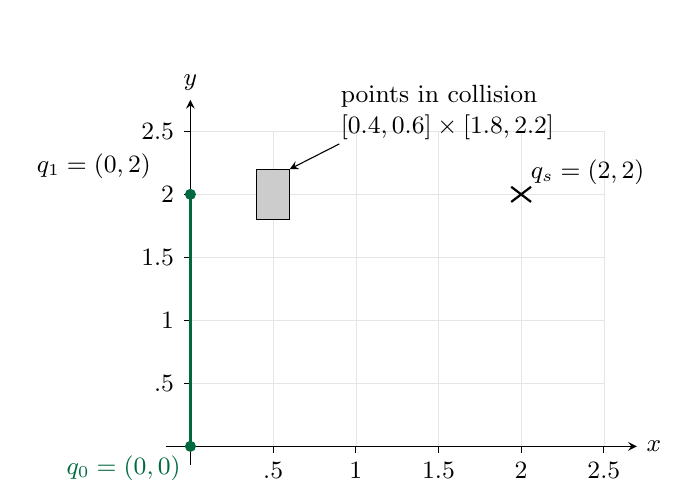
\begin{tikzpicture}[x=2.1cm,y=1.6cm,>=stealth,font=\small]
\draw[step=.5,gray!20,very thin] (0,0) grid (2.5,2.5);
\draw[->] (-.15,0)--(2.7,0) node[right]{$x$};
\draw[->] (0,-.15)--(0,2.75) node[above]{$y$};
\foreach \x in {.5,1,1.5,2,2.5}
  \draw (\x,0)--(\x,-.05) node[below]{\x};
\foreach \y in {.5,1,1.5,2,2.5}
  \draw (0,\y)--(-.04,\y) node[left]{\y};
\filldraw[fill=gray!40,draw=black] (.4,1.8) rectangle (.6,2.2);
\node[align=left,anchor=west] at (.85,2.65)
 {points in collision\\$[0.4,0.6]\times[1.8,2.2]$};
\draw[->] (.9,2.4)--(.6,2.2);
\draw[DartmouthGreen,very thick] (0,0)--(0,2);
\fill[DartmouthGreen] (0,0) circle(2pt) node[below left]{$q_0=(0,0)$};
\fill[DartmouthGreen] (0,2) circle(2pt);
\node[anchor=east] at (-.18,2.22) {$q_1=(0,2)$};
\draw[thick] (1.94,1.94)--(2.06,2.06) (1.94,2.06)--(2.06,1.94);
\node[above right] at (2,2) {$q_s=(2,2)$};
\end{tikzpicture}
\end{center}
\begin{enumerate}[label=(\alph*)]
\item Identify the nearest node and compute the proposed new node for
maximum extension length 1. Is that endpoint itself in collision?
Show your work. Check the connecting segment separately in part (b).

\begin{studentanswer}{1.0in}
%%%%% SOLUTION HERE %%%%%
\end{studentanswer}

\item For the same length-1 extension, determine whether the entire
segment from the nearest node to the proposed endpoint is collision-free.
Should RRT accept the extension? Explain why an endpoint check alone is
insufficient, and state what the tree contains after this iteration.

\begin{studentanswer}{1.1in}
%%%%% SOLUTION HERE %%%%%
\end{studentanswer}

\Needspace{3in}
\item Starting independently from the original two-node tree in each
case, compare maximum extension lengths $\tfrac14$, 1, and 2 for
the same sample. For each length, give the proposed endpoint, state
whether the endpoint is in collision, and determine whether the entire
connecting segment is collision-free. Which extensions would RRT accept?
Your length-1 result should agree with parts (a) and (b).
Does this comparison establish that a smaller or larger maximum extension
is preferable for the planning problem as a whole? Explain.

\begin{studentanswer}{1.1in}
%%%%% SOLUTION HERE %%%%%
\end{studentanswer}

\end{enumerate}

\clearpage
\section*{Question 3: Learning from recorded episodes}
A fixed policy generates the following three episodes. The state $Z$
is terminal, arrows show observed rewards, and $\gamma=\tfrac12$.
The episodes are listed in the order they were recorded.
\[
\begin{array}{c|c}
\text{Episode}&\text{Observed transitions}\\\hline
1&A\xrightarrow{2}B\xrightarrow{4}Z\\
2&A\xrightarrow{0}B\xrightarrow{2}Z\\
3&A\xrightarrow{1}B\xrightarrow{6}Z
\end{array}
\]
\begin{enumerate}[label=(\alph*)]
\item Compute the discounted return from $A$ and from $B$ in each
episode. Then compute the direct-evaluation estimate of each state's value.

\begin{studentanswer}{1.0in}
%%%%% SOLUTION HERE %%%%%
\end{studentanswer}

\item Start $V(A)=V(B)=0$ and process the transitions in their
recorded order with TD learning rate $\alpha=\tfrac12$. Keep the estimates
between episodes and hold $V(Z)=0$. For each of the six transitions,
show the sample $r+\gamma V(s')$ and the updated value of the state
being left. Give the final table.

\begin{studentanswer}{1.4in}
%%%%% SOLUTION HERE %%%%%
\end{studentanswer}

\item Explain why these estimates can differ without either
calculation being incorrect. Identify the continuation information each uses.

\begin{studentanswer}{0.7in}
%%%%% SOLUTION HERE %%%%%
\end{studentanswer}

\end{enumerate}

\clearpage
\section*{Question 4: Evaluation is not improvement}
An MDP has states $A,B,Z$, with terminal value $V(Z)=0$ and
$\gamma=\tfrac12$. At $A$, action \emph{stop} gives reward 1 and goes
to $Z$. Action \emph{continue} gives reward 0 and goes to $B$.
At $B$, the only action gives reward 4 and goes to $Z$.
All transitions are deterministic.
\begin{enumerate}[label=(\alph*)]
\item Evaluate the policy that stops at $A$. Give $V^\pi(A)$ and $V^\pi(B)$.

\begin{studentanswer}{0.65in}
%%%%% SOLUTION HERE %%%%%
\end{studentanswer}

\item Perform one policy-improvement step at $A$, showing the
value assigned to each candidate action. Does the policy change?

\begin{studentanswer}{0.7in}
%%%%% SOLUTION HERE %%%%%
\end{studentanswer}

\item Independently initialize $V_0(A)=V_0(B)=0$ and perform
two synchronous VI sweeps. Give $V_1$ and $V_2$. Explain why the first
sweep is not the same operation as exact policy evaluation followed by improvement.

\begin{studentanswer}{1.0in}
%%%%% SOLUTION HERE %%%%%
\end{studentanswer}

\end{enumerate}

\clearpage
\section*{Question 5: Descending on an approximation}
Let $f(x)=x^4-2x^2+x+1$. Consider its quadratic Taylor approximation
$m(x)$ about $x_0=1$.
\begin{enumerate}[label=(\alph*)]
\item Evaluate $f(1)$, $f'(1)$, and $f''(1)$ and construct $m(x)$.

\begin{studentanswer}{1.0in}
%%%%% SOLUTION HERE %%%%%
\end{studentanswer}

\item Starting at $x=1$, take one gradient step on $m$ with
$\alpha=\tfrac18$. Show that the result minimizes $m$, but is not a
stationary point of $f$. What does this show about interpreting a step
computed from a local model?

\begin{studentanswer}{1.3in}
%%%%% SOLUTION HERE %%%%%
\end{studentanswer}

\end{enumerate}

\clearpage
\section*{Question 6: Planning to make coffee}
A six-joint arm must move a mug around a cluttered counter. Joint limits
and a geometric collision checker are available. A new arrangement of
objects is used for each task. Consider RRT, PRM, A*, trajectory
optimization, VI, and Q-learning. More than one choice can be defended.
State the assumptions supporting your answer.
\begin{enumerate}[label=(\alph*)]
\item Propose an approach for moving the mug between two specified
arm configurations in one arrangement. Justify your choice and compare
it with a plausible alternative. State any additional assumptions your
approach requires.

\begin{studentanswer}{0.95in}
%%%%% SOLUTION HERE %%%%%
\end{studentanswer}

\item The resulting path avoids the objects, but the planned motion
changes direction abruptly and is unsuitable for carrying a full mug.
How would you revise your approach? Explain what you would change and
what evidence would be needed before accepting the revised motion.

\begin{studentanswer}{0.7in}
%%%%% SOLUTION HERE %%%%%
\end{studentanswer}

\item The robot must choose whether to fill the mug before or after
moving it. A small discrete model gives transition probabilities and
rewards, including the consequences of spills. Propose a method for
making this decision, justify it relative to an alternative, and explain
how it would fit into your overall approach to the task.

\begin{studentanswer}{0.95in}
%%%%% SOLUTION HERE %%%%%
\end{studentanswer}

\end{enumerate}

\clearpage
\section*{Question 7: Same tool position, different configurations}
A planar two-link arm has unit-length links, a fixed base at $(0,0)$,
and two revolute joints. Its configuration is $q=(\theta_1,\theta_2)$,
where the second angle is relative to the first link. Configuration
$q_A=(0,\pi/2)$ has elbow $(1,0)$ and tool position $(1,1)$.
Configuration $q_B=(\pi/2,-\pi/2)$ has elbow $(0,1)$ and the same tool
position $(1,1)$. Treat links as zero-width segments. The only obstacle
is a disk of radius $0.1$ centered at $(1,0)$.
Draw the two arm configurations as needed to support your reasoning.
\begin{enumerate}[label=(\alph*)]
\item What is the dimension of configuration space? Explain why
the tool position alone does not specify the configuration in this example.

\begin{studentanswer}{0.8in}
%%%%% SOLUTION HERE %%%%%
\end{studentanswer}

\item Which of $q_A,q_B$ is collision-free? Explain why checking
only the tool point would give an incorrect safety conclusion.

\begin{studentanswer}{1.0in}
%%%%% SOLUTION HERE %%%%%
\end{studentanswer}

\end{enumerate}

\clearpage
\section*{Question 8: Interpreting a learning experiment}
A robot follows one fixed policy and records complete episodes. Its
engineer first wants to estimate that policy's expected return, not find
a different policy. Later, the engineer trains a Q-learner using an
exploratory behavior policy and reports the reward collected during training.
\begin{enumerate}[label=(\alph*)]
\item Compare direct evaluation and TD V-learning for the
initial objective. State what each uses as a target and one reason to
prefer either method in a specified data-collection setting. Is Q-learning
with a maximizing target evaluating the same fixed policy?

\begin{studentanswer}{1.1in}
%%%%% SOLUTION HERE %%%%%
\end{studentanswer}

\item Does high or low reward during exploratory training by
itself establish how well the final greedy policy performs? Describe a
separate evaluation that would support that conclusion without changing
the learned table, and identify one limitation of the resulting evidence.

\begin{studentanswer}{1.0in}
%%%%% SOLUTION HERE %%%%%
\end{studentanswer}

\end{enumerate}

\clearpage
\section*{Question 9: What a value table cannot identify}
An agent is given a value table but no transition or reward model. Each
MDP below has one nonterminal state $s$, two actions $a,b$, and a terminal
state. Both actions terminate immediately. Rewards are deterministic.
\begin{enumerate}[label=(\alph*)]
\item Construct two such MDPs with the same $V^\pi(s)$ for
$\pi(s)=a$ and identical observed episodes under $\pi$, but different
uniquely optimal actions. Explain why arbitrarily many episodes under
that policy cannot distinguish the MDPs.

\begin{studentanswer}{1.3in}
%%%%% SOLUTION HERE %%%%%
\end{studentanswer}

\item Could exact $V^*$ alone, without a model, always identify
an optimal action? Give another pair of MDPs to establish your answer.
Explain why being given exact $Q^*$ changes the action-selection problem.

\begin{studentanswer}{1.3in}
%%%%% SOLUTION HERE %%%%%
\end{studentanswer}

\end{enumerate}
\clearpage
\section*{Question 10: Special cases of search}
\begin{enumerate}[label=(\alph*)]
\item Run A* with $\heur \equiv 0$. Which classic algorithm are you
      now running?
\item Under what \emph{two} conditions on $\heur$ and the edge costs
      does A* reduce to breadth-first search?
\end{enumerate}

\begin{studentanswer}{0.7in}
%%%%% SOLUTION HERE %%%%%
\end{studentanswer}

\newpage
\section*{Question 11: Value iteration on a chain}
Three states in a row: $s_1 \leftrightarrow s_2 \rightarrow s_3$. From $s_1$
you may move right to $s_2$ or stay. From $s_2$ you may move right into
$s_3$ or left to $s_1$. Entering $s_3$ (the goal, absorbing, $\Vfun(s_3)
\equiv 0$) earns reward $+8$. Every other transition earns 0. Discount
$\disc = 0.5$. Starting from $\Vfun_0 = 0$ everywhere, run \textbf{two}
synchronous value-iteration sweeps and give $\Vfun_1$ and $\Vfun_2$ for
$s_1$ and $s_2$.

\begin{studentanswer}{1.2in}
%%%%% SOLUTION HERE %%%%%
\end{studentanswer}

\clearpage
\section*{Question 12: Scaling a grid heuristic}
On a 4-connected unit-cost grid, consider $\heur_1 = $ Manhattan distance to
the goal and $\heur_2 = 2 \times$ Manhattan distance.

\begin{enumerate}[label=(\alph*)]
\item Which are admissible? Justify using the cell adjacent to the
      goal.
\item One sentence: what can A* return if you run it with $\heur_2$?
\end{enumerate}

\begin{studentanswer}{0.9in}
%%%%% SOLUTION HERE %%%%%
\end{studentanswer}

\clearpage
\section*{Question 13: Diagnosing controller behavior}
A point-mass robot is commanded to move to position $p=1$ m. The plots
below show its position over time for three different controller
configurations. For each plot, compare the observed behavior with the
following candidate causes:

\begin{enumerate}[label=(\arabic*)]\tightlist
\item position feedback only, no damping (no velocity or derivative term);
\item a constant disturbance (the test strip is on a slope) and no
      integral action;
\item an excessively large effort weight $\Rc$, giving weak control;
\item an excessively small effort weight $\Rc$, causing actuator saturation;
\item the reference is not reachable under the control limits.
\end{enumerate}

\begin{center}
\includegraphics[width=0.32\linewidth]{midterm-practice/figures/symptom_a.pdf}
\includegraphics[width=0.32\linewidth]{midterm-practice/figures/symptom_b.pdf}
\includegraphics[width=0.32\linewidth]{midterm-practice/figures/symptom_c.pdf}
\end{center}

\begin{enumerate}[label=(\alph*)]

\item \begin{minipage}[t]{\linewidth}
For plot A, identify the most likely cause from the list, justify the diagnosis, and propose a correction.

\begin{studentanswer}{3cm}
%%%%% SOLUTION HERE %%%%%

\end{studentanswer}

\end{minipage}

\item \begin{minipage}[t]{\linewidth}
For plot B, identify the most likely cause from the list, justify the diagnosis, and propose a correction.

\begin{studentanswer}{3cm}
%%%%% SOLUTION HERE %%%%%

\end{studentanswer}

\end{minipage}

\item \begin{minipage}[t]{\linewidth}
For plot C, identify the most likely cause from the list, justify the diagnosis, and propose a correction.

\begin{studentanswer}{3cm}
%%%%% SOLUTION HERE %%%%%

\end{studentanswer}

\end{minipage}

\end{enumerate}

\clearpage
\section*{Question 14: Policy evaluation and optimal control}
Consider finite discounted Markov decision processes with $0<\gamma<1$.
Here, V-learning means tabular TD evaluation of a fixed policy $\pi$.
Value iteration (VI) and policy iteration (PI) have access to the exact
transition and reward model; V-learning and Q-learning use sampled transitions.
All values are tabular, and terminal states have value zero. Distinguish
the information needed to learn a value function from the information
needed to select an action once that value function is known. In parts
(b) and (c), all rewards are deterministic and each action leads directly
to the terminal state. You may choose any real-valued rewards.

\begin{enumerate}[label=(\alph*)]
\item Compare VI, PI, V-learning, and Q-learning in a table or four
short paragraphs. For each method, identify the stored value function
and any explicit policy, the information used in an update, and whether
the objective is fixed-policy evaluation or optimal control. Explain
whether the successor value follows the current policy or includes a
maximization over actions. Then describe the two stages of PI and explain
why completing policy evaluation alone does not complete policy iteration.

\begin{studentanswer}{8cm}
%%%%% SOLUTION HERE %%%%%

\end{studentanswer}

\clearpage
\item A student claims: ``Once V-learning has recovered $V^\pi$ exactly,
we can identify an optimal action in every state without a transition or
reward model.'' Disprove this claim using two MDPs with one nonterminal
state $s$, two actions $a,b$, and one terminal state. Both actions terminate
immediately, and $\pi(s)=a$. Your MDPs must have the same $V^\pi(s)$ but
different uniquely optimal actions. Explain why observing only this policy
does not allow a learner to distinguish the two MDPs. State the reward
of each action in each MDP, compute $V^\pi(s)$, and identify the unique
optimal action in each. Finally, explain why additional episodes under
the same fixed policy do not resolve the ambiguity. Your argument should
concern missing information, not estimation error or slow convergence.

\begin{studentanswer}{5cm}
%%%%% SOLUTION HERE %%%%%

\end{studentanswer}

\clearpage
\item Suppose instead that the learner knows $V^*$ exactly but still has
no model. Does this resolve the problem? Construct two one-step MDPs with
the same $V^*(s)$ but different uniquely optimal actions. Then explain
what additional information lets VI and PI extract a greedy policy, and
why $Q^*$ itself is sufficient without a model. Give both reward tables,
compute the optimal values, and explicitly identify the optimal actions.
Write the model-based one-step lookahead expression used for policy
extraction and the corresponding expression when $Q^*$ is available.
Explain why being given an exact function is different from having
enough experience to learn it accurately.

\begin{studentanswer}{5cm}
%%%%% SOLUTION HERE %%%%%

\end{studentanswer}

\end{enumerate}

\clearpage
\section*{Question 15: Inflated heuristics}
A* normally prioritizes nodes using $g(n)+h(n)$. Consider a variant
that gives the heuristic twice as much weight and instead uses
\[ f_2(n)=g(n)+2h(n). \]
At each step, it removes a node with the smallest $f_2$ from the frontier.
It returns a path when the goal is removed, not when the goal is first
discovered. As in the other search questions, it reopens an expanded
node if a lower-cost path to that node is found.

All edge costs are positive. Let $C^*$ be the cost of an optimal path
from the start to the goal. The heuristic is admissible and satisfies
$h(G)=0$. Write $g^*(n)$ for the optimal cost from the start to $n$ and
$h^*(n)$ for the optimal remaining cost from $n$ to the goal.

You may use the following fact without proving it. Immediately before
the algorithm removes the goal, some node $n$ on an optimal path is
still on the frontier with $g(n)=g^*(n)$.

\begin{enumerate}[label=(\alph*)]
\item Prove that $f_2(n)\le2C^*$ for the frontier node
described above. Justify the inequalities in your argument.

\begin{studentanswer}{8cm}
%%%%% SOLUTION HERE %%%%%
\end{studentanswer}

\end{enumerate}

\clearpage
\section*{Part 2: Programming practice}
The starter code is in \texttt{midterm-practice/code/}. Complete the
two learning modules, then run the provided experiment and public checks
from the course repository root. The checks are available for practice,
not as an additional PS2 requirement.
\begin{verbatim}
python midterm-practice/code/autograder.py
\end{verbatim}
\subsection*{Task 1: Learning from experience}

\textbf{Connection to PS2.} PS2 P2 evaluates a fixed policy from recorded
transitions. PS2 P3 examines what Q-learning can learn when exploration
does not reach an important reward. This task implements both settings
on the same grid-MDP interface used in PS1.

In \texttt{passive\_rl.py}, implement \texttt{direct\_evaluation} and
\texttt{td\_evaluation}. The runner supplies completed episodes generated
by a fixed policy on a small course-grid environment. Direct evaluation
averages the discounted return from every visit to a state. TD evaluation
processes the same transitions in chronological order, updating only the
state being left. Initialize values to zero, keep terminal values at zero,
and follow the supplied function contracts. Neither method changes the policy.

In \texttt{q\_learning.py}, implement tabular Q-learning with
$\epsilon$-greedy exploration. For an observed transition $(s,a,r,s')$,
use
\[
\text{sample}=r+\gamma\max_{a'}Q(s',a'),\qquad
Q(s,a)\leftarrow(1-\alpha)Q(s,a)+\alpha\,\text{sample}.
\]
At a terminal transition, use $\text{sample}=r$. With probability
$\epsilon$, select a uniformly random action; otherwise select a greedy
action, resolving ties in N, S, E, W order. Use only the supplied random
generator, in the draw order specified in the starter. Record the training
statistics using the provided \texttt{Stats} class.

Run \texttt{python midterm-practice/code/run\_learning.py}. The first experiment
compares direct and TD estimates from the same fixed-policy episodes.
The second trains Q-learning on open, maze, and narrow using the settings
in \texttt{constants.py}, then tests each greedy policy. The runner also
repeats the maze experiment without exploration. The known model is used
by the runner for evaluation only; neither learning implementation may
inspect the transition model beyond the sampled transitions it receives
or, for Q-learning, its calls to \texttt{world.step}.

\textbf{Files to complete.} Implement \texttt{passive\_rl.py} and
\texttt{q\_learning.py}. Record the results below in your practice PDF.

\clearpage
\textbf{PDF responses.}
\begin{enumerate}[label=(\alph*)]
\item \begin{minipage}[t]{\linewidth}
Include \texttt{practice\_learning.png}, comparing the two passive estimates
with the fixed policy's exact values. Explain in two sentences why
finite-data estimates may differ even though the episodes are identical.

\begin{studentanswer}{9cm}
%%%%% SOLUTION HERE %%%%%
\end{studentanswer}

\end{minipage}
\item \begin{minipage}[t]{\linewidth}
Include the Q-learning results table. Report goal-reaching performance
and the greedy path length for each map, including the no-exploration
maze run. Explain the latter result using PS2 P3, and distinguish evaluating
a fixed policy from learning action values for policy improvement.

\begin{studentanswer}{7cm}
%%%%% SOLUTION HERE %%%%%
\end{studentanswer}

\end{minipage}
\end{enumerate}


\ifdefined\CUMULATIVEPRACTICE
\else
\end{document}
\fi
